\documentclass{article}
\usepackage[utf8]{inputenc}
\usepackage[T1]{fontenc}
\usepackage[export]{adjustbox}
\usepackage{mathtools,amsthm,amssymb,icomma,upgreek,xfrac,enumerate, bbm,titlesec,lmodern,polski,derivative,geometry,multicol,titling,graphicx,url,amsmath,caption,lipsum,float,longtable,booktabs}
\usepackage[table,xcdraw]{xcolor}
\usepackage[hidelinks,breaklinks,pdfusetitle,pdfdisplaydoctitle]{hyperref}
\usepackage{listings}
\definecolor{codegreen}{rgb}{0,0.6,0}
\definecolor{codegray}{rgb}{0.5,0.5,0.5}
\definecolor{codepurple}{rgb}{0.58,0,0.82}
\definecolor{backcolour}{rgb}{0.95,0.95,0.92}
\definecolor{light-gray}{gray}{0.95}
\setlength{\droptitle}{-1cm}
\mathtoolsset{showonlyrefs,mathic}
\title{Komputerowa analiza szeregów czasowych raport 1}
\author{Natalia Klepacka, Joanna Kołaczek}
\date{21.12.2022}
\newtheoremstyle{break}
{\topsep}{\topsep}%
{\normalfont}{}%
{\bfseries}{}%
{\newline}{}%
\theoremstyle{break}

\titleformat*{\section}{\LARGE\bfseries}
\titleformat*{\subsection}{\Large\bfseries}
\titleformat*{\subsubsection}{\large\bfseries}
\titleformat*{\paragraph}{\large\bfseries}
\titleformat*{\subparagraph}{\large\bfseries}

\lstdefinestyle{mystyle}{
	backgroundcolor=\color{backcolour},   
	commentstyle=\color{codegreen},
	keywordstyle=\color{magenta},
	numberstyle=\tiny\color{codegray},
	stringstyle=\color{codepurple},
	basicstyle=\ttfamily\footnotesize,
	breakatwhitespace=false,         
	breaklines=true,                 
	captionpos=b,                    
	keepspaces=true,                 
	numbers=left,                    
	numbersep=5pt,                  
	showspaces=false,                
	showstringspaces=false,
	showtabs=false,                  
	tabsize=2
}

\lstset{style=mystyle}
\renewcommand{\lstlistingname}{Kod}% Listing -> Kod
\renewcommand{\lstlistlistingname}{Lista Kodów}% List of Listings -> Lista kodów
\newcommand{\code}[1]{\colorbox{light-gray}{\texttt{#1}}}

\graphicspath{{obrazki/}}


\begin{document}
	\maketitle
	\tableofcontents
	\clearpage
\section{Wstęp}
	Niniejszy raport powstał na potrzeby realizacji laboratorium z Komputerowej Analizy Szeregów Czasowych, prowadzonych przez mgr Justynę Witulską, do wykładu prof. Agnieszki Wyłomańskiej.
	Będziemy analizować dane dotyczące poziomu szczęścia w wybranych krajach na świecie oraz jego związku z wartością PKB na osobę (w dalszej części raportu, będziemy je określać skrótowo jako szczęście i PKB). Po usunięciu wartości brakujących dysponujemy próbami o wielkości~791. Dane pochodzą \href{https://www.kaggle.com/datasets/eliasturk/world-happiness-based-on-cpi-20152020}{\textit{z tej strony}}. Są to wyniki uzyskane przez Instytut Gallupa, w ankietach badających poziom szczęścia oraz jego możliwe indykatory, zebrane  w latach 2015-2020. W raporcie przeprowadzimy analizę jednowymiarową dla dwóch zmiennych oraz zwizualizujemy je przy pomocy histogramu, dystrybuanty empirycznej oraz boxplotu. Następnie wyestymujemy współczynniki w klasycznym modelu regresji, aby ostatecznie sprawdzić, czy uzyskane residua spełniają oczekiwane założenia.
	
	Życzymy Czytelnikowi miłej lektury.
	
\section{Analiza jednowymiarowa zmiennej zależnej oraz zmiennej niezależnej}

\subsection{Wizualizacja danych}

W przeprowadzanej przez nas analizie zmienną zależną jest \textbf{szczęście}, natomiast zmienną niezależną jest \textbf{PKB}. Rozkład danych możemy zobaczyć na histogramach [\ref{fig:hist}]. Zauważmy, że rozkład szczęścia wydaje się bardziej symetryczny niż rozkład PKB, który sprawia wrażenie lewoskośnego. Jednakże, niestety na pierwszy rzut oka, nie przypominają nam one żadnego ze znanych rozkładów.

\begin{figure}[H]
	\begin{center}
		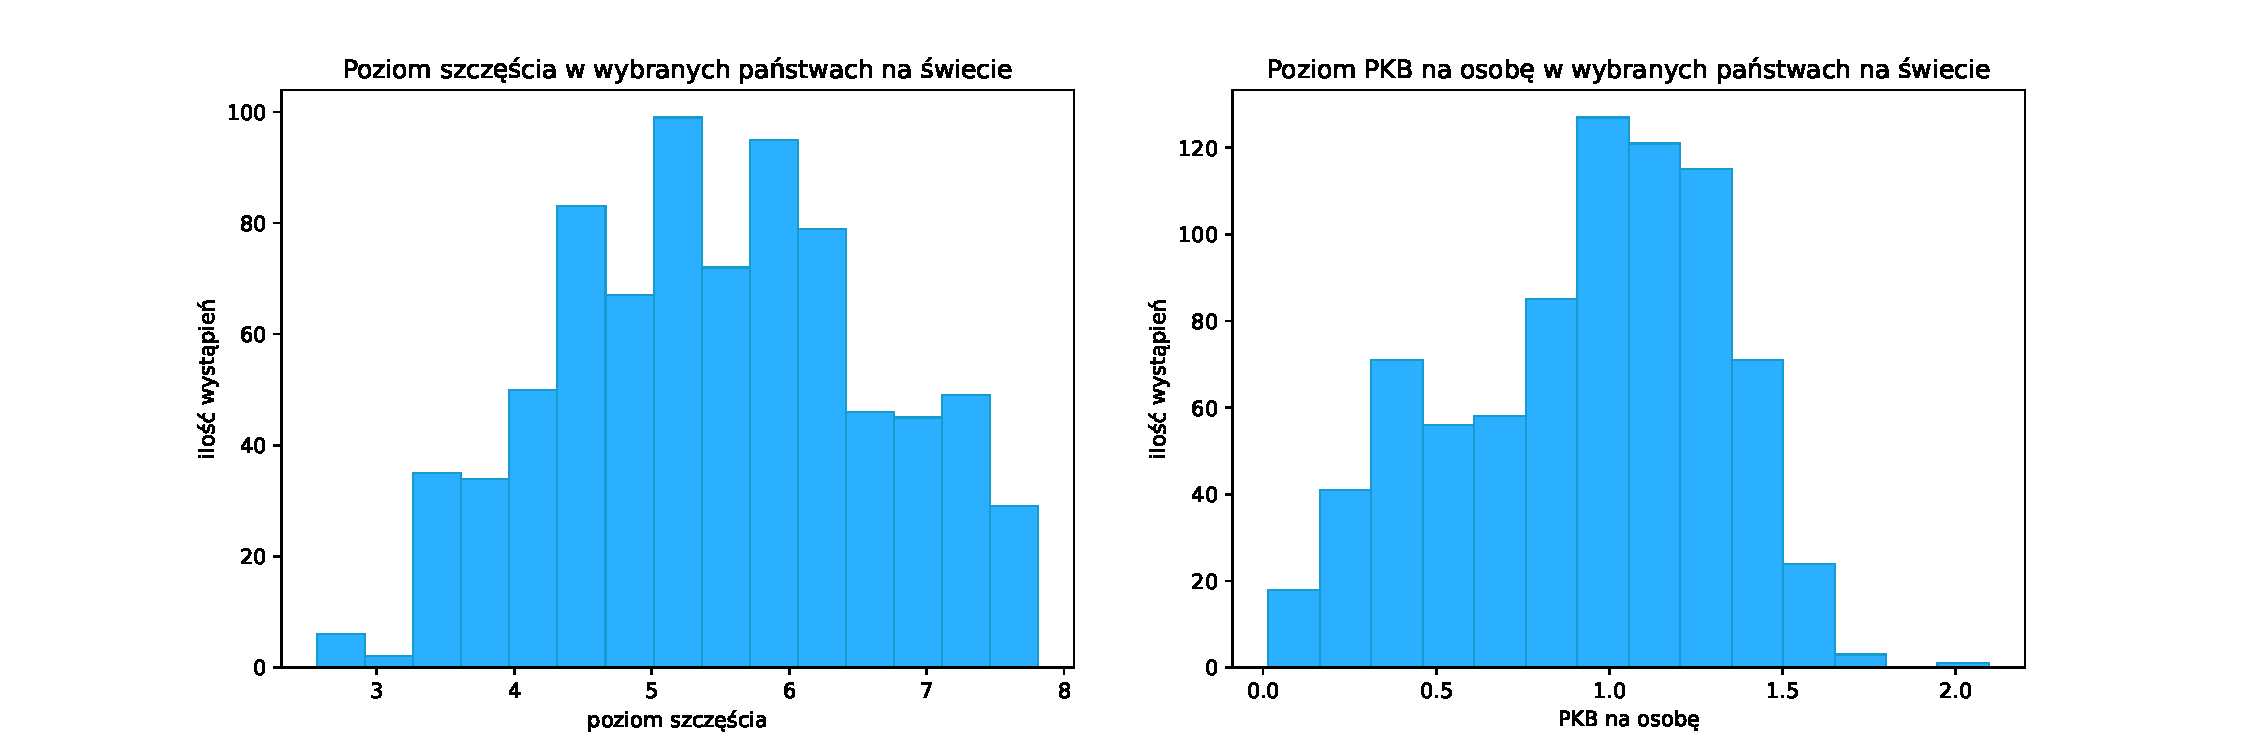
\includegraphics[scale=0.43]{hist.pdf}
		\caption{Histogramy}
		\label{fig:hist}
	\end{center}
\end{figure}

Dystrybuanty empiryczne [\ref{fig:distr}] pokazują, z jakim prawdopodobieństwem natrafimy na kolejno szczęście i PKB mniejsze bądź równe od danej wartości. Gdy spojrzymy na dystrybuantę szczęścia, wydaje się, że ma ona ogony lżejsze niż rozkład normalny. Dystrybuanta PKB, tak jak jego histogram, nie jest symetryczna. 

\begin{figure}[H]
	\begin{center}
		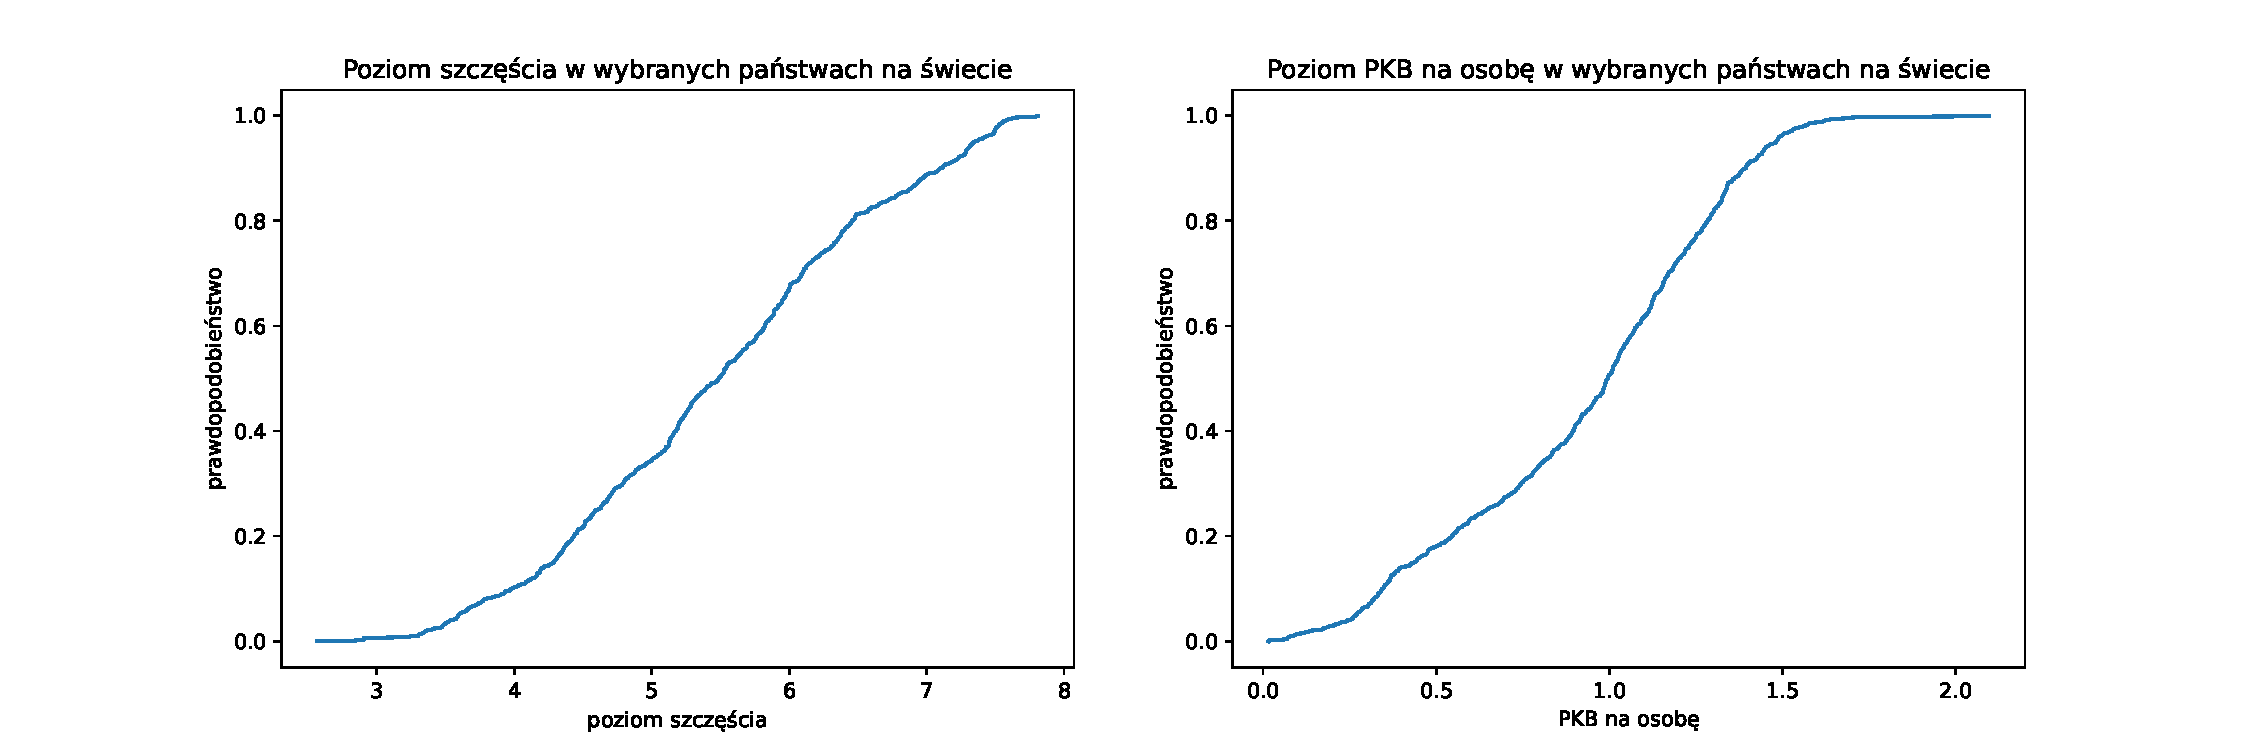
\includegraphics[scale=0.43]{distr.pdf}
		\caption{Dystrybuanta empiryczna}
		\label{fig:distr}
	\end{center}
\end{figure}

Wykres pudełkowy (ang. \textit{boxplot}) [\ref{fig:box}] jest to graficzna reprezentacja mediany oraz kwartyli. Końce wąsów wskazują ostatnią wartość odległą od końca "pudełka" o co najwyżej półtorej wartości rozstępu międzykwartylowego. Co ciekawe, w naszych danych nie pojawiły się wartości odstające, zatem możemy sądzić, że dane zostały rzetelnie zebrane, a ryzyko przeprowadzenia błędnej analizy (nieodzwierciedlającej rzeczywistych trendów) jest mniejsze.

\begin{figure}[H]
	\begin{center}
		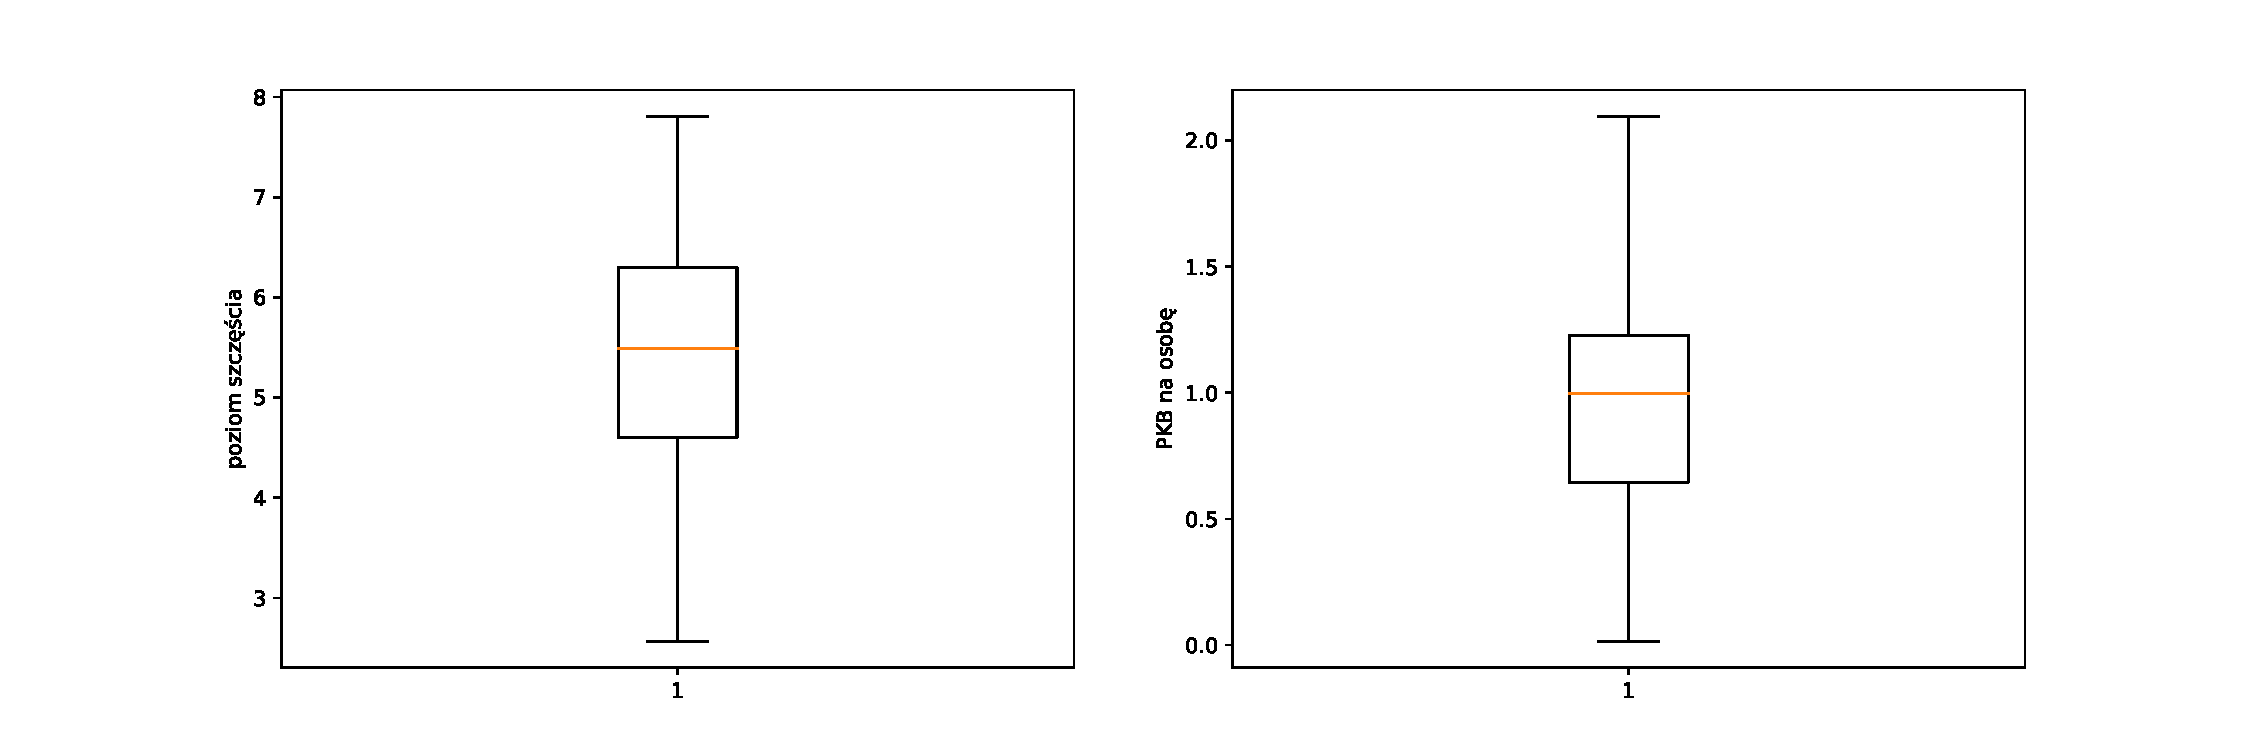
\includegraphics[scale=0.43]{box.pdf}
		\caption{Boxploty}
		\label{fig:box}
	\end{center}
\end{figure}

\subsection{Podstawowe miary}

W tabeli [\ref{table}] podsumowałyśmy najistotniejsze miary położenia, rozproszenia, spłaszczenia i skośności. Rzeczywiście skośność, którą odczytałyśmy z histogramu PKB, jest ujemna (zatem rozkład jest lewoskośny), natomiast skośność szczęścia jest niewielka. Przypuszczenia z wykresu dystrybuanty empirycznej również się sprawdziły --- kurtoza szczęścia jest mniejsza od 3 więc rozkład ten jest platokurtyczny. 


\begin{table}[H]
	\centering
	\begin{tabular}{|ll|l|l|}
		\hline
		\rowcolor[HTML]{C0C0C0} 
		\multicolumn{2}{|l|}{\cellcolor[HTML]{C0C0C0}Miary}                             & Poziom szczęścia & PKB na osobe \\ \hline
		\multicolumn{1}{|l|}{}                               & średnia arytmetyczna     & 5.47             & 0.93         \\ \cline{2-4} 
		\multicolumn{1}{|l|}{}                               & średnia geometryczna     & 5.23             & 0.58         \\ \cline{2-4} 
		\multicolumn{1}{|l|}{}                               & średnia harmoniczna      & 5.35             & 0.81         \\ \cline{2-4} 
		\multicolumn{1}{|l|}{}                               & średnia ucinana 10\%     & 5.47             & 0.94         \\ \cline{2-4} 
		\multicolumn{1}{|l|}{}                               & mediana Q2               & 5.48             & 0.99         \\ \cline{2-4} 
		\multicolumn{1}{|l|}{}                               & Q1                       & 4.59             & 0.64         \\ \cline{2-4} 
		\multicolumn{1}{|l|}{położenia}    & Q3                       & 6.30             & 1.22         \\ \hline
		\multicolumn{1}{|l|}{}                               & rozstęp                  & 5.24             & 2.08         \\ \cline{2-4} 
		\multicolumn{1}{|l|}{}                               & rozstęp międzykwartylowy & 1.70             & 0.58         \\ \cline{2-4} 
		\multicolumn{1}{|l|}{}                               & wariancja nieobciążona   & 1.26             & 0.14         \\ \cline{2-4} 
		\multicolumn{1}{|l|}{}                               & odchylenie standardowe   & 1.12             & 0.38         \\ \cline{2-4} 
		\multicolumn{1}{|l|}{rozproszenia} & współczynnik zmienności  & 20.52            & 41.33        \\ \hline
		\multicolumn{1}{|l|}{spłaszczenia}                   & kurtoza                  & 2.25             & 2.31         \\ \hline
		\multicolumn{1}{|l|}{skośności}                      & skośność                 & -0.01            & -0.36        \\ \hline
	\end{tabular}
\caption{Zestawienie statystyk.}
\label{table}
\end{table}
	
\section{Analiza zależności liniowej pomiędzy zmienną zależną a zmienną niezależną}

\subsection{Wykres rozproszenia i określenie zależności}

\begin{figure}[H]
	\begin{center}
		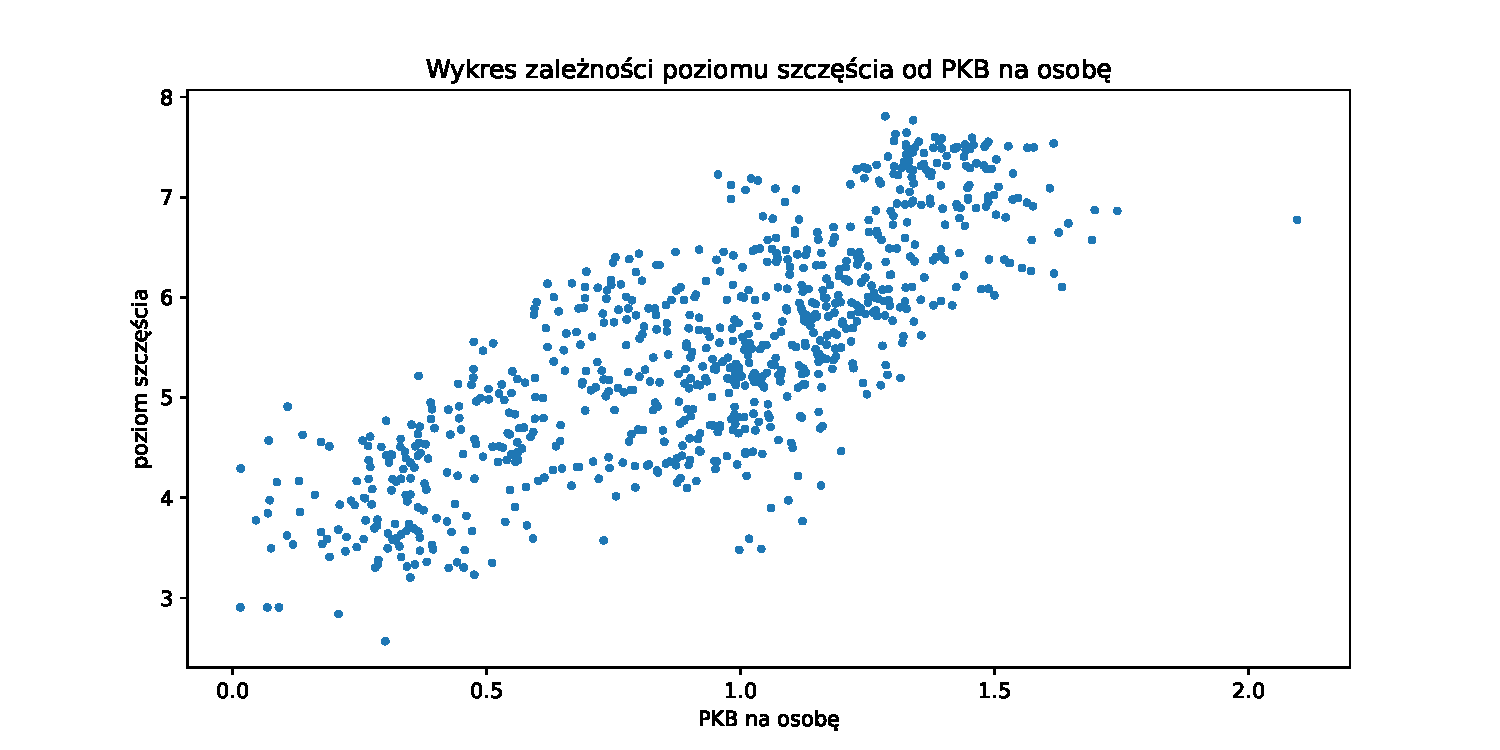
\includegraphics[scale=0.43]{plot1.pdf}
		\caption{Wykres rozproszenia}
		\label{fig:rozproszenie}
	\end{center}
\end{figure}

Na podstawie wykresu rozproszenia [\ref{fig:rozproszenie}] możemy stwierdzić, że zależność pomiędzy zmiennymi prawdopodobnie jest liniowa.

\subsection{Punktowa estymacja współczynników}

Współczynniki regresji liniowej wyliczamy ze wzorów
\begin{equation}
\left\{ \begin{array}{ll}
	\hat{\beta}_{1} = r\frac{S_{y}}{S_{x}}\\
	\hat{\beta}_{0} = \bar{y} - r\beta_{1}\bar{x}
\end{array} \right.,
\label{eq:wspol_reg}
\end{equation} gdzie
\begin{equation}
	r = \frac{1}{n-1}\frac{\sum_{i=1}^{n}(x_i-\bar{x})(y_i-\bar{y})}{S_{x}S_{y}},
\end{equation}
\begin{equation}
	S_{x} = \sqrt{\frac{1}{n-1}\sum_{i=1}^{n}(x_{i}-\bar{x})^{2}},
\end{equation}
\begin{equation}
	S_{y} = \sqrt{\frac{1}{n-1}\sum_{i=1}^{n}(y_{i}-\bar{y})^{2}},
\end{equation}
\begin{equation}
	\bar{x} = \frac{1}{n}\sum_{i=1}^{n}x_{i},
\end{equation}
\begin{equation}
	\bar{y} = \frac{1}{n}\sum_{i=1}^{n}y_{i}.
\end{equation}

Wzory te zostały wyznaczone przy pomocy metody najmniejszych kwadratów.

\begin{figure}[H]
	\begin{center}
		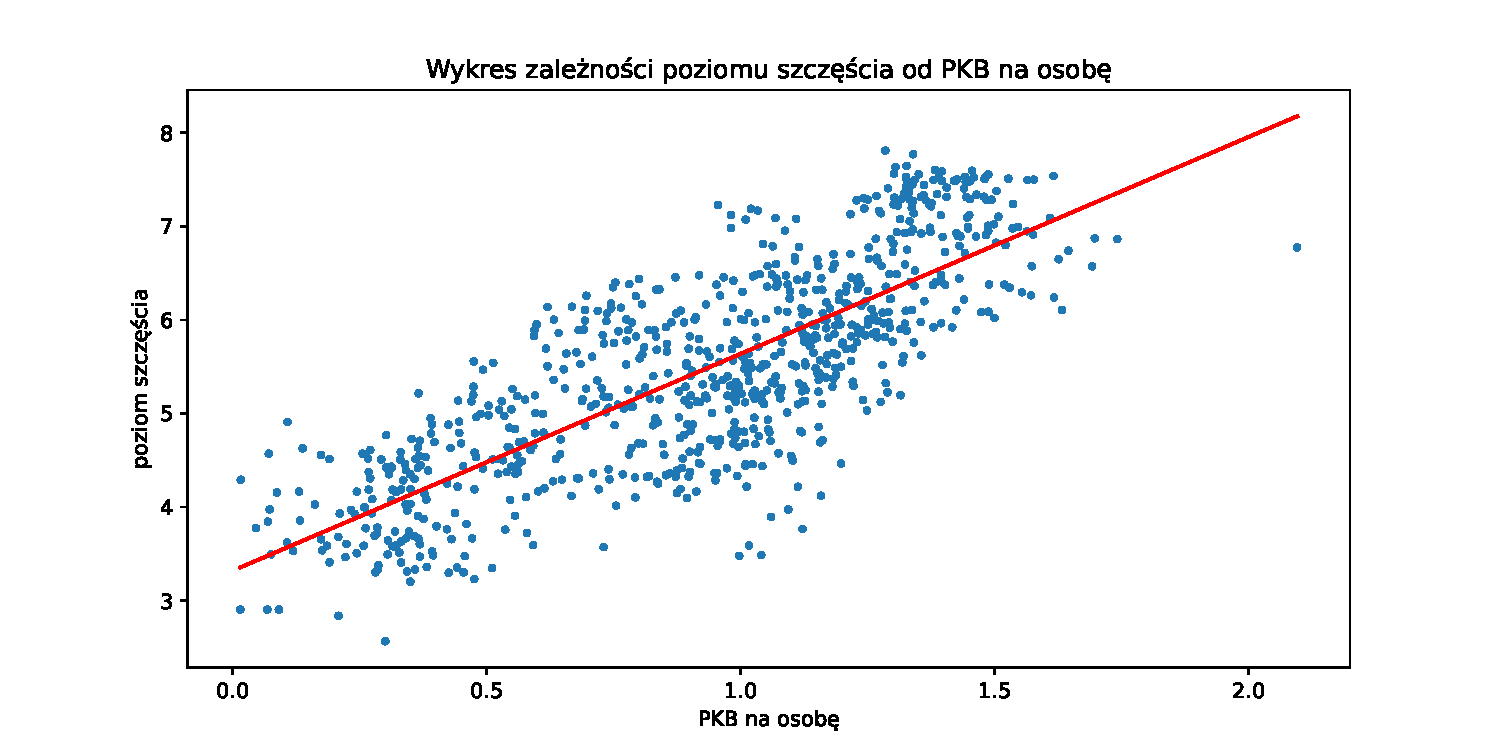
\includegraphics[scale=0.43]{plot2.pdf}
		\caption{Wykres rozproszenia z zaznaczoną prostą regresji}
		\label{fig:prosta}
	\end{center}
\end{figure}

Z powyższych wzorów otrzymaliśmy współczynniki o wartościach
\begin{equation}
	\left\{ \begin{array}{ll}
		\hat{\beta}_{1} \approx 2.32\\
		\hat{\beta}_{0} \approx 3.32
	\end{array} \right..
\end{equation}
Współczynniki te opisują prostą widoczną na wykresie [\ref{fig:prosta}].

\subsection{Przedziałowa estymacja współczynników}

Z założenia o normalności rozkładu $\{\varepsilon\}_{i=1}^{n}$, przy braku znajomości jego wariancji możemy stwierdzić, że unormowane parametry $\beta_0$, $\beta_1$ mają rozkład t-studenta z n-2 stopniami swobody. Przedziały ufności przyjmują wtedy postać
\begin{equation}
\left\{ \begin{array}{ll}
	P\left(\hat{\beta}_{0}-t_{n-2}(1-\frac{\alpha}{2})S\sqrt{\frac{1}{n}+\frac{\bar{x}^{2}}{\sum_{i=1}^{n}(x_i-\bar{x})^2}} < \beta_{0} < \hat{\beta}_{0}+t_{n-2}(1-\frac{\alpha}{2})S\sqrt{\frac{1}{n}+\frac{\bar{x}^{2}}{\sum_{i=1}^{n}(x_i-\bar{x})^2}}\right) = 1-\alpha\\
	P\left(\hat{\beta}_{1}-t_{n-2}(1-\frac{\alpha}{2})\frac{S}{\sqrt{\sum_{i=1}^{n}(x_i-\bar{x})^2}} < \beta_{1} < \hat{\beta}_{1}+t_{n-2}(1-\frac{\alpha}{2})\frac{S}{\sqrt{\sum_{i=1}^{n}(x_i-\bar{x})^2}}\right) = 1-\alpha
\end{array} \right.,
\end{equation} gdzie
\begin{equation}
	S = \sqrt{\frac{\sum_{i=1}^{n}(y_i - \hat{y}_i)^2}{n-2}}.
\end{equation}
Przyjmując $\alpha = 0.05$ otrzymujemy zatem, że z 95\% prawdopodobieństwem
\begin{equation}
	\left\{ \begin{array}{ll}
		\beta_{1} \in (2.19, 2.44)\\
		\beta_{0} \in (3.20, 3.44)
	\end{array} \right..
\end{equation}

\subsection{Ocena poziomu zależności}

Poziom zależności liniowej pomiędzy zmiennymi można ocenić przy pomocy wielu różnych współczynników. Jednym z nich jest współczynnik korelacji Pearsona
\begin{equation}
	r = \frac{1}{n-1}\frac{\sum_{i=1}^{n}(x_i-\bar{x})(y_i-\bar{y})}{S_{x}S_{y}},
\end{equation}
gdzie
\begin{equation}
S_{x} = \sqrt{\frac{1}{n-1}\sum_{i=1}^{n}(x_{i}-\bar{x})^{2}},
\end{equation}
\begin{equation}
S_{y} = \sqrt{\frac{1}{n-1}\sum_{i=1}^{n}(y_{i}-\bar{y})^{2}},
\end{equation}

W opisywanym przypadku współczynnik ten przyjmuje wartość $r \approx 0.79$, co oznacza, że w danych występuje dosyć silna pozytywna zależność liniowa.
 
Jakość dopasowania modelu możemy sprawdzić też przy pomocy współczynników SST, SSE i SSR.
\begin{equation}
	SST = \sum_{i=1}^{n}\left(y_i-\bar{y}\right)
\end{equation}
\begin{equation}
	SSE = \sum_{i=1}^{n}\left(y_i-\hat{y}_i\right)
\end{equation}
\begin{equation}
	SSR = \sum_{i=1}^{n}\left(\hat{y}_i-\bar{y}\right)
\end{equation}
Wiemy, że $SST = SSR + SSE$. Ponadto im mniejsze $SSE$, a zarazem $SSR$ bliższe $SST$, tym lepiej dopasowany jest model. W opisywanym przypadku otrzymaliśmy $SST \approx 997.74$, $SSE \approx 370.75$, oraz $SSR \approx 626.98$. Jak widać, $SSE$ jest znacząco mniejsze od $SSR$, zatem nasz model jest dosyć dobrze dopasowany do danych.
\subsection{Predykcja oraz jej przedziały ufności}

W tej części wykonamy predykcję wartości zmiennej zależnej dla 20 największych obserwacji zmiennej niezależnej. W tym celu estymujemy współczynniki ze wzorów [\ref{eq:wspol_reg}], używając jednak tylko 771 obserwacji. Otrzymujemy w ten sposób 
\begin{equation}
	\left\{ \begin{array}{ll}
		\beta_{1} \approx 2.36\\
		\beta_{0} \approx 3.29
	\end{array} \right..
\end{equation}
Następnie wartości dla ostatnich 20 obserwacji wyliczamy ze wzoru $\hat{Y}_0 = \hat{\beta}_0 + \hat{\beta}_{1}x_0$. Przy założeniu, że residua modelu mają rozkład normalny o nieznanej wariancji, możemy stwierdzić, że przedziały ufności dla $Y_0$ przyjmują postać
\begin{equation}
	P\left(\hat{Y}_0 - t_{n-2}\left(1-\frac{\alpha}{2}\right)S\sqrt{1+\frac{1}{n}+\frac{(x_0-\bar{x}_n)^2}{\sum_{i=1}^{n}(x_i - \bar{x}_n)^2}} \leqslant Y_0 \leqslant \hat{Y}_0 + t_{n-2}\left(1-\frac{\alpha}{2}\right)S\sqrt{1+\frac{1}{n}+\frac{(x_0-\bar{x}_n)^2}{\sum_{i=1}^{n}(x_i - \bar{x}_n)^2}}\right) = 1-\alpha.
\end{equation}
Rezulaty powyższej procedury można zobaczyć na wykresie [\ref{fig:predykcja}].

\begin{figure}[H]
	\begin{center}
		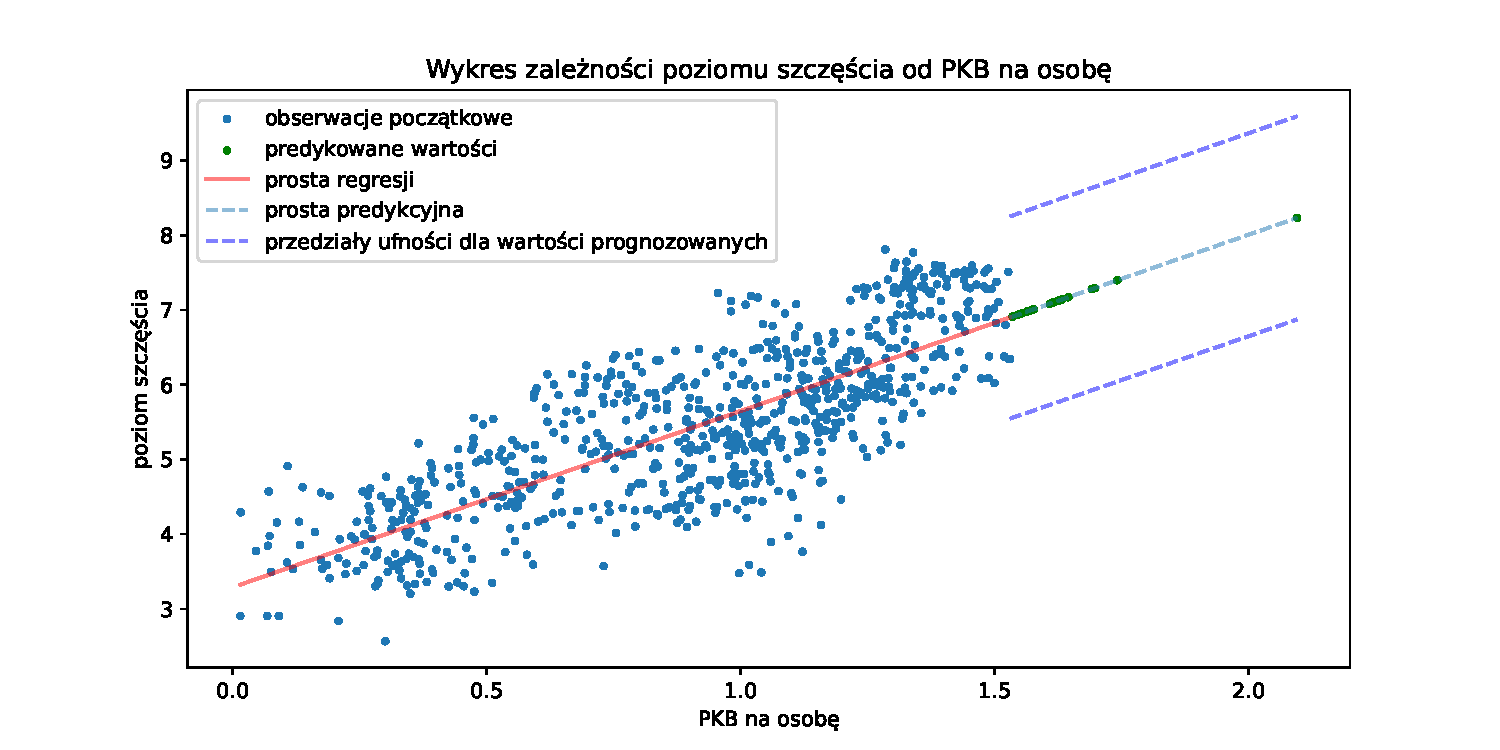
\includegraphics[scale=0.6]{pred.pdf}
		\caption{Predykcja dla ostatnich 20 obserwacji zmiennej niezależnej}
		\label{fig:predykcja}
	\end{center}
\end{figure}

\section{Analiza residuów}
\subsection{Wstęp}

W tej części przeprowadzimy analizę residuów. Dzięki temu możemy ocenić czy model regresji liniowej jest dobrym wyborem dla naszego zbioru danych. Pod nazwą residuum mamy na myśli różnicę między wartością wyestymowaną a rzeczywistą.

\begin{equation}
	e_i = y_i - \hat(y)_i
\end{equation}

W klasycznym modelu regresji zakładamy, że residua mają średnią równą 0, stałą wariancję, są niezależne od siebie nawzajem i mają rozkład normalny.

\subsection{Średnia i wariancja}
\begin{figure}[H]
	\begin{center}
		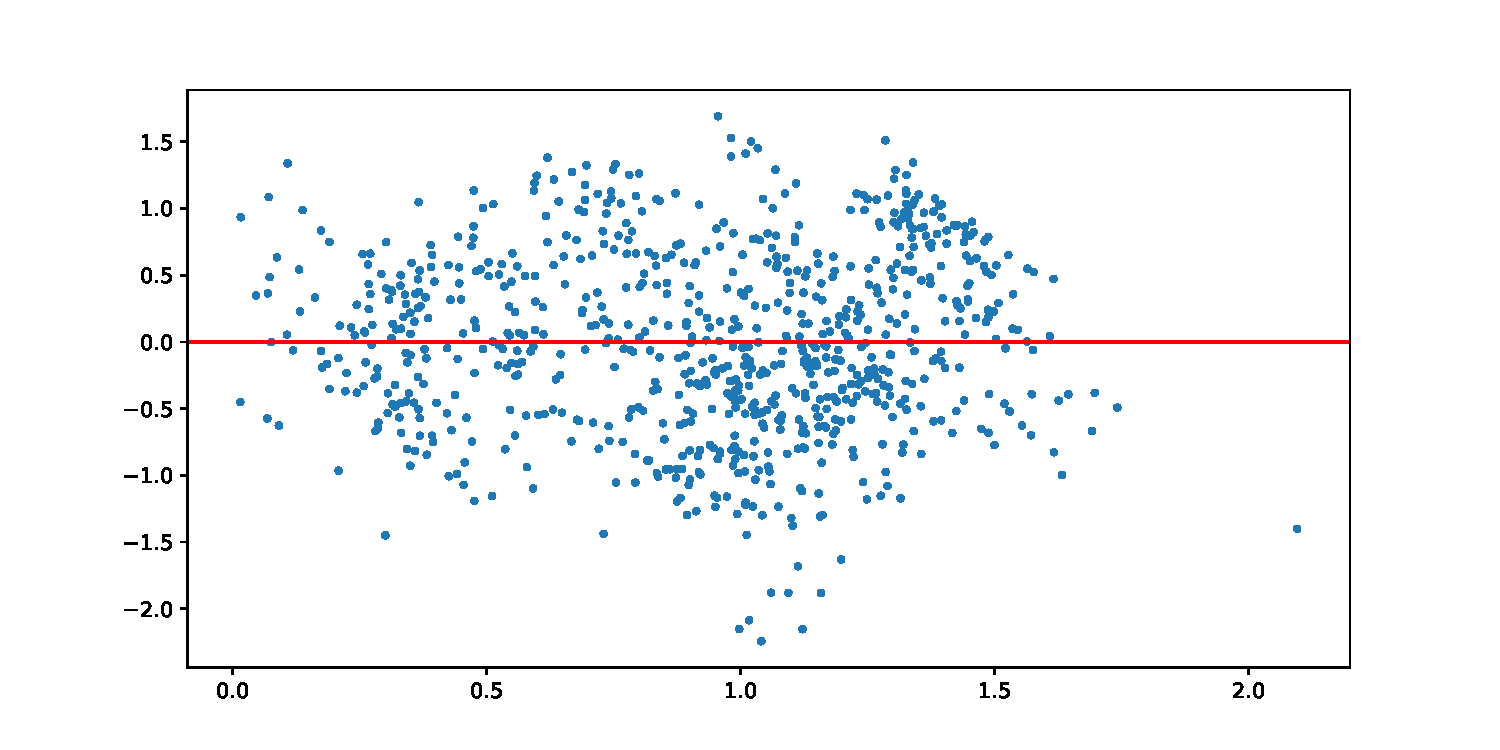
\includegraphics[scale=0.5]{res.pdf}
		\caption{Residua}
		\label{fig:res}
	\end{center}
\end{figure}

Na wykresie [\ref{fig:res}] przedstawione zostały residua z regresji liniowej szczęścia w zależności od PKB. Czerwona linia oznacza średnią, która jest bliska zeru. Na pierwszy rzut oka widzimy, że wariancja jest raczej równa na całej długości osi zmiennej niezależnej. Aby upewnić się, czy nasze przewidywanie jest słuszne, wykonamy test Levene'a jednorodności wariancji [\ref{levene}]. 

\begin{lstlisting}[language=Python, caption=Test Levene'a, label={levene}]
	stat, p_value = scipy.stats.levene(random.sample(residuals,350),random.sample(residuals,350))
	if p_value > 0.05:
		print("Wariancja jest raczej stala.")
	else:
		print("Wariancja raczej nie jest stala.")
		
	#output
	Wariancja jest raczej stala.
\end{lstlisting}

Po wykonaniu testu nie mamy podstaw, aby odrzucić hipotezę zerową: "Wszystkie próbki są z populacji o równej wariancji". 

\subsection{Niezależność}

Następnie będziemy chciały sprawdzić, czy residua są niezależne. Ponieważ na wykresie [\ref{fig:res}] trudno dostrzec zależność, wykonamy test Durbina-Watsona [\ref{durbin}].

\begin{lstlisting}[language=Python, caption=Test Durbina-Watsona, label={durbin}]
	from statsmodels.stats.stattools import durbin_watson as dwtest
	dwtest(resids=np.array(residuals))
	
	#output
	1.2617265161048754
\end{lstlisting}

Jeżeli wynik jest bliski 2, oznacza to, że residua nie są skorelowane, jeżeli natomiast jest mniejszy od 1 lub większy od 3, korelacja z dużym prawdopodobieństwem występuje. W naszym przypadku test nie stwierdza jednoznacznie korelacji, sugeruje dodatnią korelację, co możemy również zobrazować na wykresie [\ref{fig:acor}], który wykorzystuje funkcję \code{acf} z pakietu \code{statsmodels.tsa.stattools}, aby policzyć autokorelację.

\begin{figure}[H]
	\begin{center}
		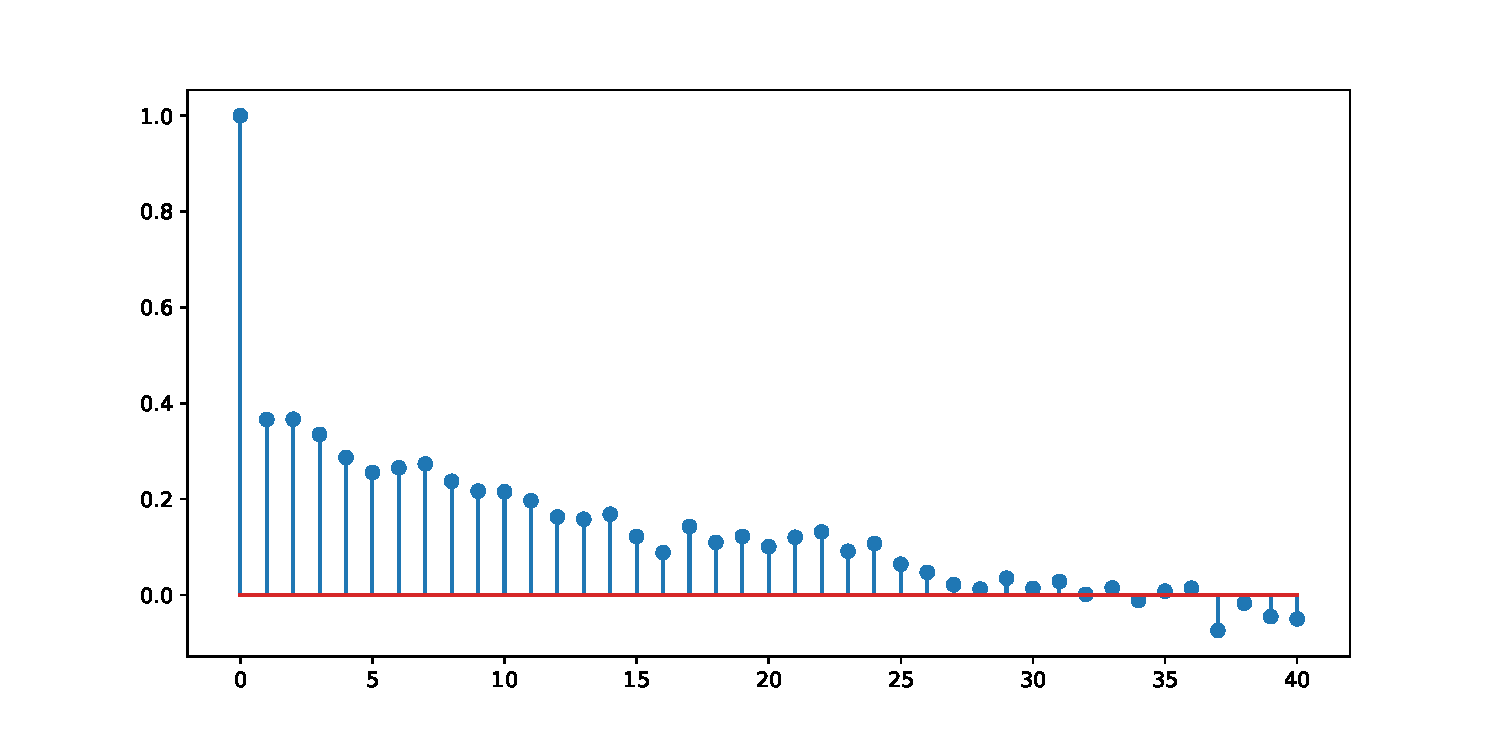
\includegraphics[scale=0.5]{acor.pdf}
		\caption{Autokowariancja residuów}
		\label{fig:acor}
	\end{center}
\end{figure}

\subsection{Normalność rozkładu}

Na koniec, sprawdzimy jeszcze, czy rozkład residuów jest normalny. W tym celu porównamy ich histogram z gęstością rozkładu normalnego [\ref{fig:res_hist}]. 
\begin{figure}[H]
	\begin{center}
		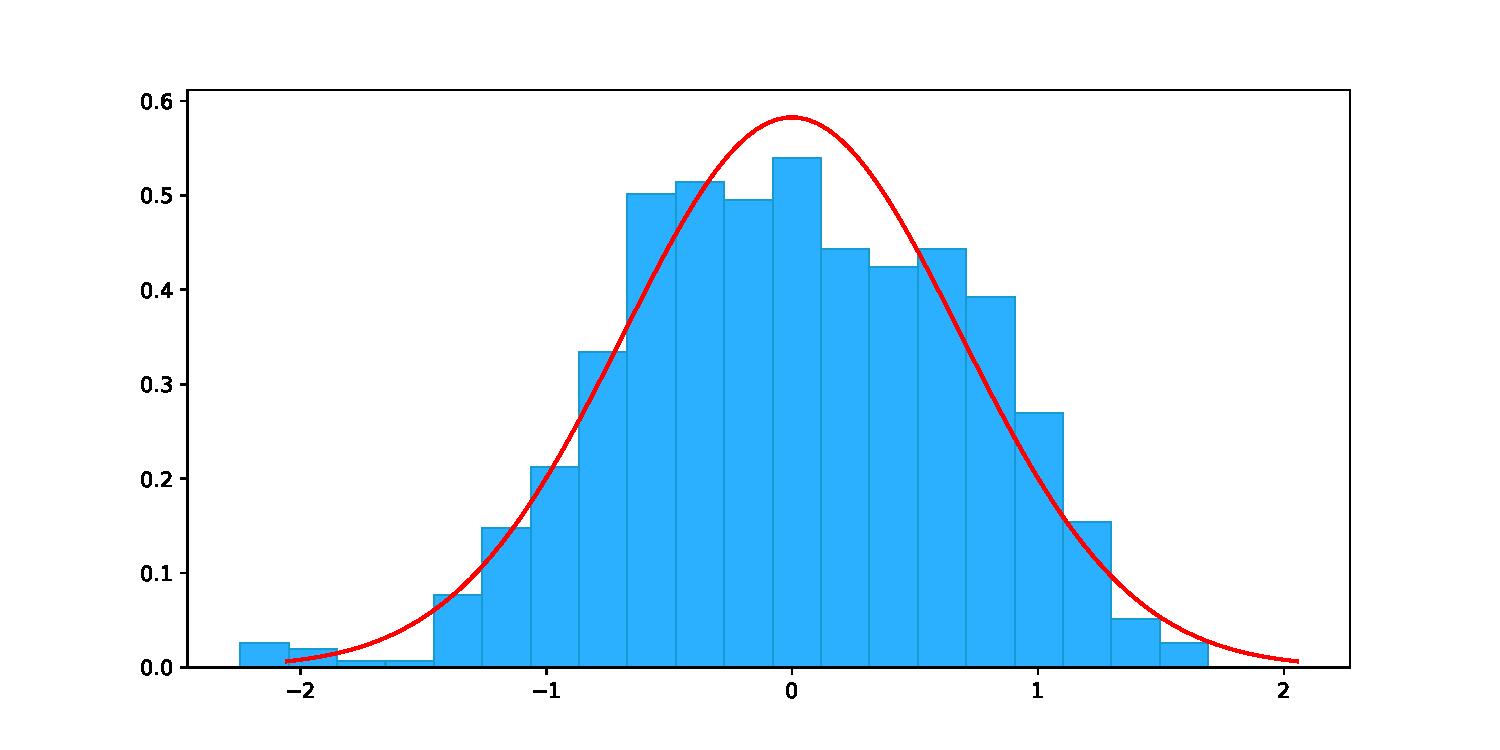
\includegraphics[scale=0.5]{res_hist.pdf}
		\caption{Rozkład residuów}
		\label{fig:res_hist}
	\end{center}
\end{figure}

 Ponieważ możemy mieć wątpliwości wynikające z różnic na wykresie, wykonamy test na normalność [\ref{norm}], który potwierdza, że residua prawdopodobnie nie mają oczekiwanego rozkładu.

\begin{lstlisting}[language=Python, caption=Test Levene'a, label={norm}]
	stat, p = scipy.stats.normaltest(residuals)
	if p > 0.05:
		print('Dane raczej pochodza z rozkladu normalnego')
	else:
		print('Dane raczej nie pochodza z rozkladu normalnego')
		
	#output
	Dane raczej nie pochodza z rozkladu normalnego
\end{lstlisting}

	
\section{Podsumowanie}

Na podstawie przeprowadzonej analizy możemy stwierdzić, że między poziomem szczęścia a PKB per capita dla danego kraju występuje dosyć silna zależność liniowa. Niestety badanie residuów wykazało, że nie mają one rozkładu normalnego. Oznacza to, że co prawda punktowe estymacje zostały przez nas wykonane poprawnie, jednak wszystkie estymacje przedziałowe oparte były o założenie o normalności rozkładu residuów, zatem nie mają zastosowania w tym modelu. Niestety nie znając rozkładu $\epsilon$, nie możemy wyznaczyć faktycznych przedziałów ufności.
	
	\section{Źródła}
	\begin{itemize}
		\item Wykłady
		\item \url{https://www.kaggle.com/datasets/eliasturk/world-happiness-based-on-cpi-20152020}
	\end{itemize}
	
	
\end{document}